\section{Human experiments of category learning}
\label{sec: experiment}

The review board of our institution provided ethical approval for all the human experiments listed below. All participants received monetary compensation above the local minimum wage for their participation.

\subsection{Methods}
We designed a categorization learning task that encourages participants to explore a four-dimensional feature space of novel visual stimuli. Each stimulus was a line drawing, parametrized by four variable-length segments with fixed angles (Fig. \ref{fig:1}A). Participants were trained to perform correct categorization following three different rules of increasing complexity (Fig. \ref{fig:1}B, between-subject design): (1) a two-category rule based on a single randomly assigned feature (e.g., leg); (2) a four-category rule requiring integration of three features(e.g., leg, tail, and head), with the hierarchical structure disclosed; and (3) a structurally similar four-category rule, but without revealing the underlying hierarchy (see Appendix A for rule details). Illustrated using the two-category task, each trial (Task 1 in Fig. \ref{fig:1}C) required participants to classify a randomly generated stimulus into one of two arbitrary categories (“F” or “J”), following a deterministic rule unknown to them. After each response, participants verbally reported the features they used to make the choice, serving as a ground truth for internal processing. Feedback was then provided (1 = correct, 0 = incorrect), followed by the next trial. Learning concluded once participants achieved over 90\% accuracy across 64 consecutive trials. Before learning, all participants completed a calibration task to quantify their baseline perceptual noise (see Appendix A).

\begin{figure}[t]  % [t] 表示让浮动体靠近页面顶部
    \centering
    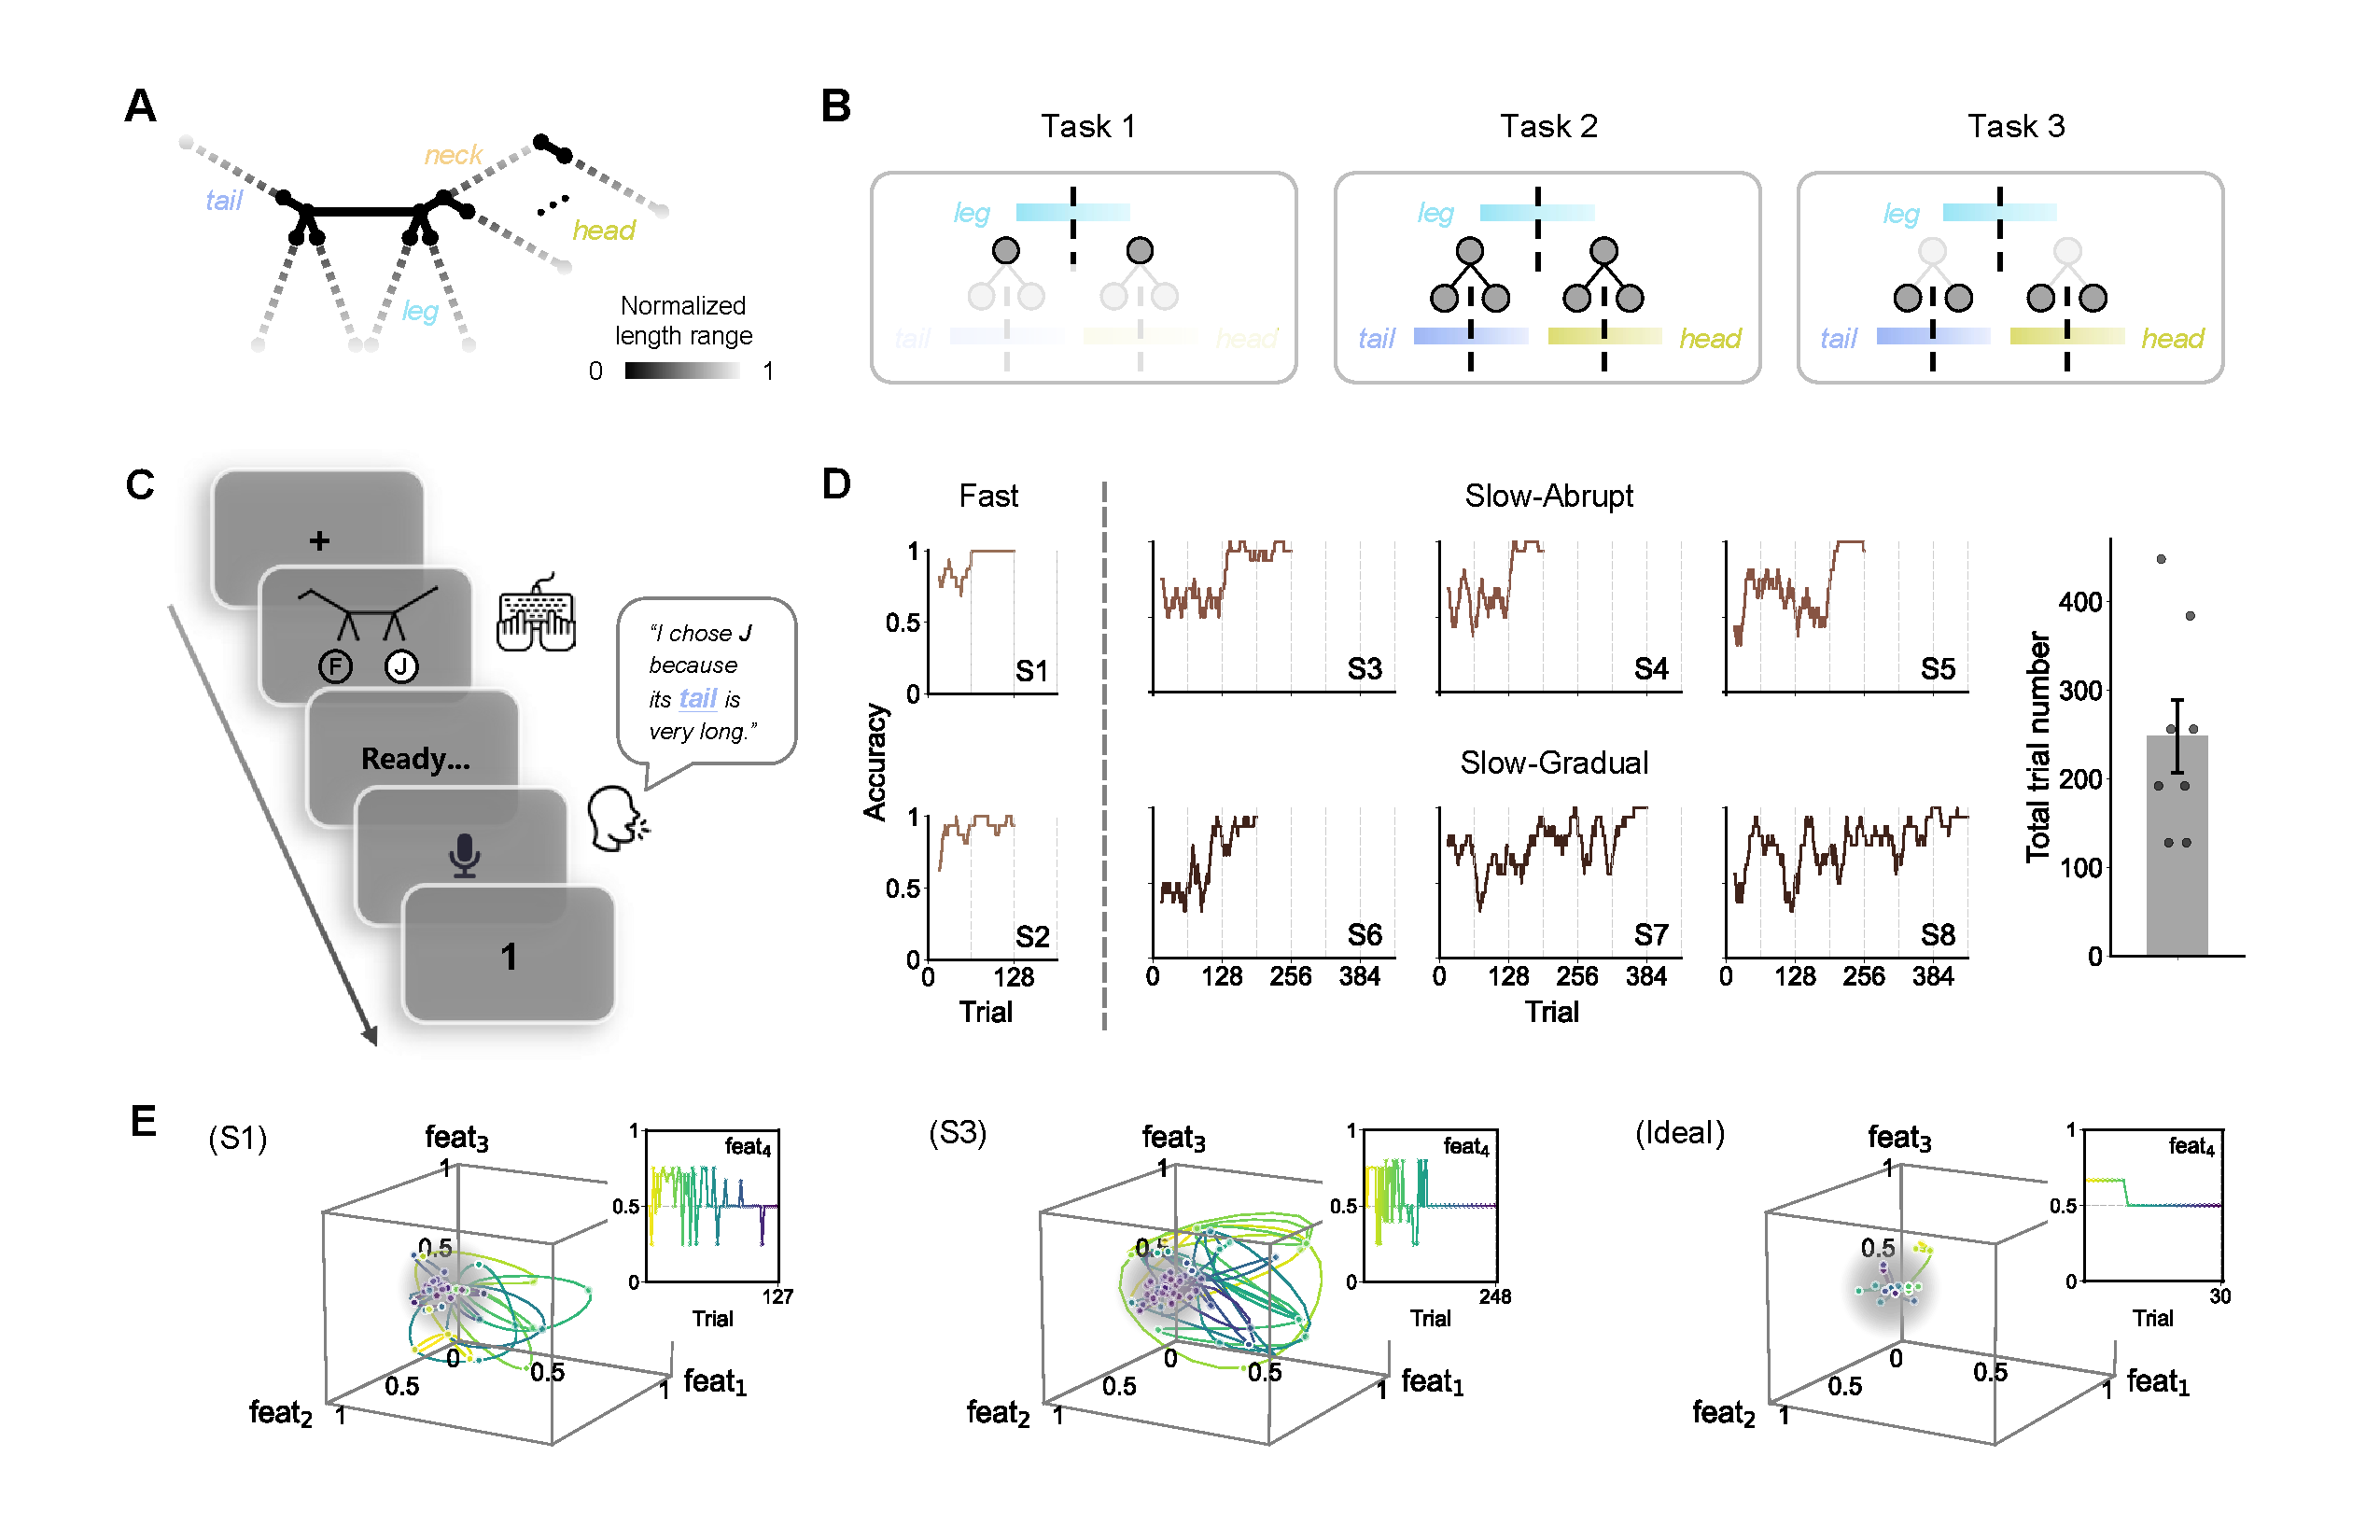
\includegraphics[width=1\textwidth, trim=0cm 0.5cm 0cm 1.5cm, clip]{figs/Figure1.pdf}
    \caption{Stimuli, task, and human behaviors. \textbf{(A)} Each stimulus has four independent length features normalized to the range 0–1. \textbf{(B)} Between-subjects tasks increase in complexity: Task 1 (two categories, single feature); Task 2 (four categories, three-feature hierarchy shown); Task 3 (same rule as Task 2, hierarchy hidden). \textbf{(C)} On each trial, participants observed a randomly sampled stimulus, selected a category (e.g., F or J in Task 1), verbally reported the feature(s) that informed their choice (indicated by a speech bubble), and received deterministic feedback. \textbf{(D)} Learning performance in Task 1 showed large individual differences: participants varied widely in the total number of trials needed to reach criterion and in sliding-window accuracy (line plots), which could be broadly classified into three groups--fast (lightest brown), slower but abrupt (medium brown), and slower and gradual (darkest brown). \textbf{(E)} Exploration trajectories in feature space from two representative participants (S1, S3) trained on the same task rule illustrate early broad sampling followed by late local refinement (as shown by the yellow-to-purple gradient), whereas the model-derived ideal observer (right) converges rapidly.}
    \label{fig:1}
\end{figure}

\subsection{Results}
Participants generally succeeded in all three tasks, with three excluded due to persistent failures. However, the number of trials needed for successful learning varied considerably across individuals within the same task (Fig. \ref{fig:1}D, boxplot). More notably, learning dynamics--quantified using sliding-window accuracy--also differed markedly: even in the simplest two-category task, participants ranged from gradual learners (lighter hues) to those exhibiting abrupt transitions (darker hues) (Fig. \ref{fig:1}D). Similar variability was observed in other more complex tasks (see Appendix A). 

To probe internal processing, we analyzed participants’ verbal reports projected into the four-dimensional stimulus space (see Appendix A for methodological details). Feature-based trajectories from two exemplar participants trained on the same rule are shown in Fig. \ref{fig:1}E (left and middle), from earlier (yellowish) to late (darkish) trials. This visualization reveals two key observations: (1) an early phase of broad, saltatory exploration, followed by a later phase of localized refined exploration; (2) substantial individual variability in these dynamics, which diverge markedly from an ideal observer (Fig. \ref{fig:1}E, right)--implemented via the baseline model described in Section \ref{sec:3.1}--who integrates evidence optimally and converges rapidly on the correct rule.

\textbf{Summary.} Our findings reveal idiosyncratic learning patterns across participants, evident in both observable performance (Fig. \ref{fig:1}D) and internal hypothesis trajectories (Fig. \ref{fig:1}E). A detailed analysis of feature exploration suggests a strategic process--participants appear to engage in active inference via simplified prior assumptions and iterative hypothesis testing--reflected in the shift from saltatory to localized sampling. Notably, these trajectories often diverged from the optimal path, underscoring the bounded rationality of human information processing. Together, these results highlight the necessity of modeling internal dynamics to uncover the underlying mechanisms of human learning. 
